\documentclass[11pt,letterpaper]{article}

\usepackage[margin=1in]{geometry}
\usepackage{graphicx}
\usepackage{booktabs}
\usepackage{multirow}
\usepackage{xcolor}
\usepackage{amsmath}
\usepackage{caption}
\usepackage{microtype}
\usepackage{hyperref}
\usepackage[numbers,sort&compress]{natbib}
\usepackage{enumitem}

\hypersetup{colorlinks=true, linkcolor=blue!50!black, citecolor=blue!50!black, urlcolor=blue!50!black}

\setlength{\parskip}{4pt}
\setlength{\parindent}{0pt}

\title{\textbf{Comparing Interpretable Sequence Features and Protein Language Models for Missense Variant Classification}}
\author{Georgios Ioannou (gi2100) \and Vedant Jagtap (vsj7589)\\\small \texttt{AI in Genomics, Spring 2026}}
\date{}

\begin{document}
\maketitle

\vspace{-1.6em}

\section*{Background}
A \emph{genetic variant} is a place in a person's DNA that differs from the human reference. We focus on \emph{missense variants}: single-letter changes in DNA that swap one amino acid for another in the resulting protein. Some missense variants disrupt protein function and cause disease (\emph{pathogenic}); others are tolerated (\emph{benign}). Deciding which is which is a central problem in clinical genetics. \textbf{ClinVar}~\citep{landrum2020clinvar,ncbi2026intro} is the largest open archive of clinical variant interpretations and is the primary data source we use.

\textbf{ESM-2}~\citep{rives2021biological,lin2023esm2} is a \emph{protein language model}: a transformer trained on hundreds of millions of natural protein sequences to predict masked amino acids. After training, ESM-2 produces a \emph{residue embedding}, a 1280-dimensional numeric vector that summarizes a residue's evolutionary and structural context. We extract that vector at the mutated position and use it as input to a small classifier.

We report \textbf{AUROC} (area under the ROC curve), \textbf{AUPRC} (area under the precision-recall curve), and \textbf{F1} (harmonic mean of precision and recall) on a \textbf{gene-held-out} test set: every gene the model is evaluated on was withheld from training, so the metrics measure \emph{cross-gene generalization} rather than memorization.

\section*{Motivation}
Many strong missense pathogenicity predictors already exist, so our goal is \emph{not} to beat the state of the art. Instead we ask two empirical questions about the gene-held-out setting: (i) how much pathogenicity signal is captured by simple, interpretable handcrafted sequence features, and (ii) whether residue embeddings from a pretrained protein language model improve cross-gene generalization beyond those features. The answers shape the four-dimensional tradeoff the proposal flagged among \emph{interpretability, computational simplicity, predictive performance, and cross-gene generalization}.

\section*{Methods}

\paragraph{Data.}
We use NCBI's ClinVar \texttt{variant\_summary.txt} (release dated \textbf{2026-05-04}, the snapshot pinned in \texttt{data/processed/clinvar\_release.txt})~\citep{ncbi2026ftp}. We restrict to GRCh38 germline single-nucleotide missense variants whose ClinVar review status maps to a clear binary label: pathogenic / likely-pathogenic vs.\ benign / likely-benign~\citep{ncbi2026clinsig,ncbi2026reviewstatus}. We exclude conflicting and uncertain interpretations. Duplicates (same RefSeq transcript, position, ref AA, alt AA) are dropped, keeping the strongest review status. Table~\ref{tab:funnel} reports the per-stage retention counts. We map each retained variant to a \emph{reviewed} (Swiss-Prot) human protein sequence in UniProt UP000005640~\citep{uniprot2026proteome}, requiring that the residue at the variant position in the canonical sequence equals the HGVS-reported reference amino acid. After this verification we retain \textbf{193{,}483} variants across \textbf{14{,}893} genes (62{,}241 pathogenic / 131{,}242 benign). Figure~\ref{fig:pipeline} sketches the full pipeline.

\paragraph{Splits.}
To prevent \emph{train--test contamination across variants of the same gene}, we use a \textbf{gene-disjoint} 70/10/20 train/val/test split (seed 42), stratified across genes by majority label so neither split is all-positive or all-negative. Final split sizes: \textbf{train 135{,}418 / val 19{,}539 / test 38{,}526} variants, with 10{,}425 / 1{,}489 / 2{,}979 unique genes respectively.

\paragraph{Models.}
We train and compare three of our own models, plus AlphaMissense~\citep{cheng2023alphamissense} and CADD~\citep{rentzsch2019cadd} as external reference points (not targets to outperform). Per the instructions, for each of our models we state input, architecture, and training data:
\begin{itemize}[leftmargin=18pt,itemsep=2pt,topsep=2pt]
\item \textbf{Logistic regression / Random forest baselines.}
  \emph{Input}: a 62-dimensional handcrafted vector per variant -- one-hot reference AA (20-d), one-hot alternate AA (20-d), BLOSUM62 substitution score (1-d), local sequence-window AA composition with radius 7 (20-d), and normalized residue position (1-d).
  \emph{Architecture}: scikit-learn \texttt{LogisticRegression} (L2, \texttt{class\_weight=balanced}, C tuned on val) and \texttt{RandomForestClassifier} (500 trees, \texttt{class\_weight=balanced}, depth and leaf grid tuned on val).
  \emph{Training data}: the 135{,}418 train variants.
\item \textbf{ESM-2 head}.
  \emph{Input}: the ESM-2 (650M, \texttt{facebook/esm2\_t33\_650M\_UR50D}) hidden state at the mutated residue (1280-d). For proteins longer than ESM-2's 1022-residue positional limit we tile the sequence with overlapping windows and pick, per variant, the tile that places it closest to the tile center.
  \emph{Architecture}: a small MLP \texttt{1280 $\to$ 256 $\to$ 1} with LayerNorm, dropout 0.2, GELU activation, sigmoid output.
  \emph{Training data}: the same 135{,}418 train variants. The ESM-2 backbone is \emph{frozen}; only the head is trained, with AdamW, cosine LR schedule, BCE-with-logits, class weighting, and early stopping on val AUPRC.
\end{itemize}
\textbf{ESM-2 caveat (proposal-flagged).} ESM-2 was pretrained on UR50, which contains many human proteins; this could inflate metrics on genes already well-represented in pretraining. We surface this caveat here and analyze it empirically in the appendix (Figure~\ref{fig:studiedness}). \textbf{Computational simplicity} is reported per model in Appendix Table~\ref{tab:efficiency}.

\paragraph{Evaluation.}
We report AUROC, AUPRC, F1, accuracy, precision, recall, and confusion matrices on the held-out test set. F1 is computed at the threshold that maximizes F1 on the validation set. 95\% confidence intervals come from a non-parametric bootstrap with 1000 resamples over test variants. The same metrics are computed for AlphaMissense and CADD on the matched intersection of test variants (Phase 10 implementation; full details in \texttt{src/imc/eval/external.py}).

\section*{Results}

\textbf{Both empirical questions answered by the numbers in Table~\ref{tab:results}.}
The interpretable handcrafted random forest reaches test AUROC $= 0.850$ and AUPRC $= 0.764$ -- it captures \emph{about 91\% of the ESM-2 head's AUROC} and \emph{85\% of its AUPRC} on a strictly cross-gene test set. ESM-2 then closes the remaining gap: the head improves AUROC by \textbf{$+0.089$} (95\% bootstrap CI excludes zero) and AUPRC by \textbf{$+0.137$}, with non-overlapping CIs against both baselines. AlphaMissense remains the strongest reference point (AUROC $0.966$); the ESM-2 head and CADD bracket it from below (Figure~\ref{fig:rocpr}).

\textbf{The advantage holds at the gene level} (Figure~\ref{fig:pergene}). Per-gene AUROCs computed on the 247 test genes with at least 5 pathogenic and 5 benign variants show the ESM-2 head's per-gene median climbing well above both baselines, with a tighter spread, despite every test gene being unseen during training.

\textbf{Errors are concentrated on the same boundary cases} (Figure~\ref{fig:confusion}). The ESM-2 head's confusion matrix shows balanced precision (0.800) and recall (0.841), whereas the LR baseline trades precision for recall (0.552 / 0.782) and the RF is balanced but lower-recall (0.637 / 0.754).

\begin{table}[t]
\centering
\small
\caption{\textbf{Test-set metrics with 95\% bootstrap confidence intervals.} All n's refer to the held-out gene-disjoint test set. F1 uses the val-tuned operating threshold. AlphaMissense covers 97.3\% of test variants; coverage of CADD is 100\%.}
\label{tab:results}
\begin{tabular}{lrlllr}
\toprule
\textbf{Model} & \textbf{n} & \textbf{AUROC [95\% CI]} & \textbf{AUPRC [95\% CI]} & \textbf{F1 [95\% CI]} & \textbf{Acc.} \\
\midrule
Logistic regression  & 38{,}526 & 0.800 [0.796, 0.805] & 0.668 [0.659, 0.677] & 0.647 [0.641, 0.653] & 0.708 \\
Random forest        & 38{,}526 & 0.850 [0.846, 0.854] & 0.764 [0.757, 0.771] & 0.691 [0.684, 0.697] & 0.768 \\
ESM-2 head           & 38{,}526 & \textbf{0.939 [0.936, 0.941]} & \textbf{0.901 [0.897, 0.906]} & \textbf{0.820 [0.815, 0.825]} & \textbf{0.874} \\
\midrule
AlphaMissense (ref.) & 37{,}736 & 0.966 [0.964, 0.967] & 0.939 [0.935, 0.942] & 0.871 [0.867, 0.876] & 0.912 \\
CADD (ref.)          & 38{,}526 & 0.928 [0.925, 0.931] & 0.839 [0.832, 0.846] & 0.807 [0.803, 0.812] & 0.860 \\
\bottomrule
\end{tabular}
\end{table}

\begin{figure}[t]
\centering
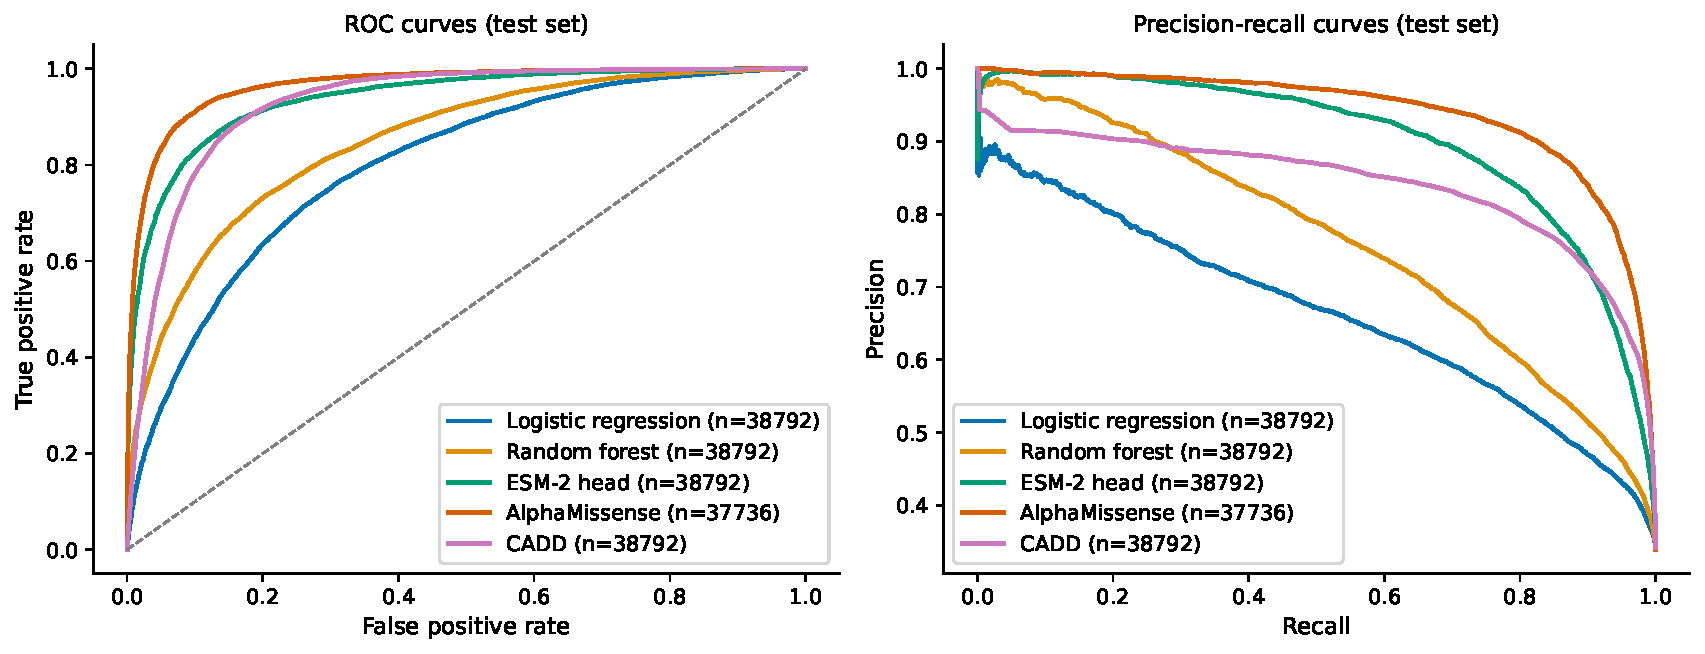
\includegraphics[width=\linewidth]{../figures/fig2_roc_pr.pdf}
\caption{\textbf{Test-set ROC and PR curves (Figure 2).} All models on $n=38{,}526$ gene-held-out test variants (AlphaMissense on 37{,}736 with score coverage). The ESM-2 head sits between the handcrafted baselines and AlphaMissense.}
\label{fig:rocpr}
\end{figure}

\begin{figure}[t]
\centering
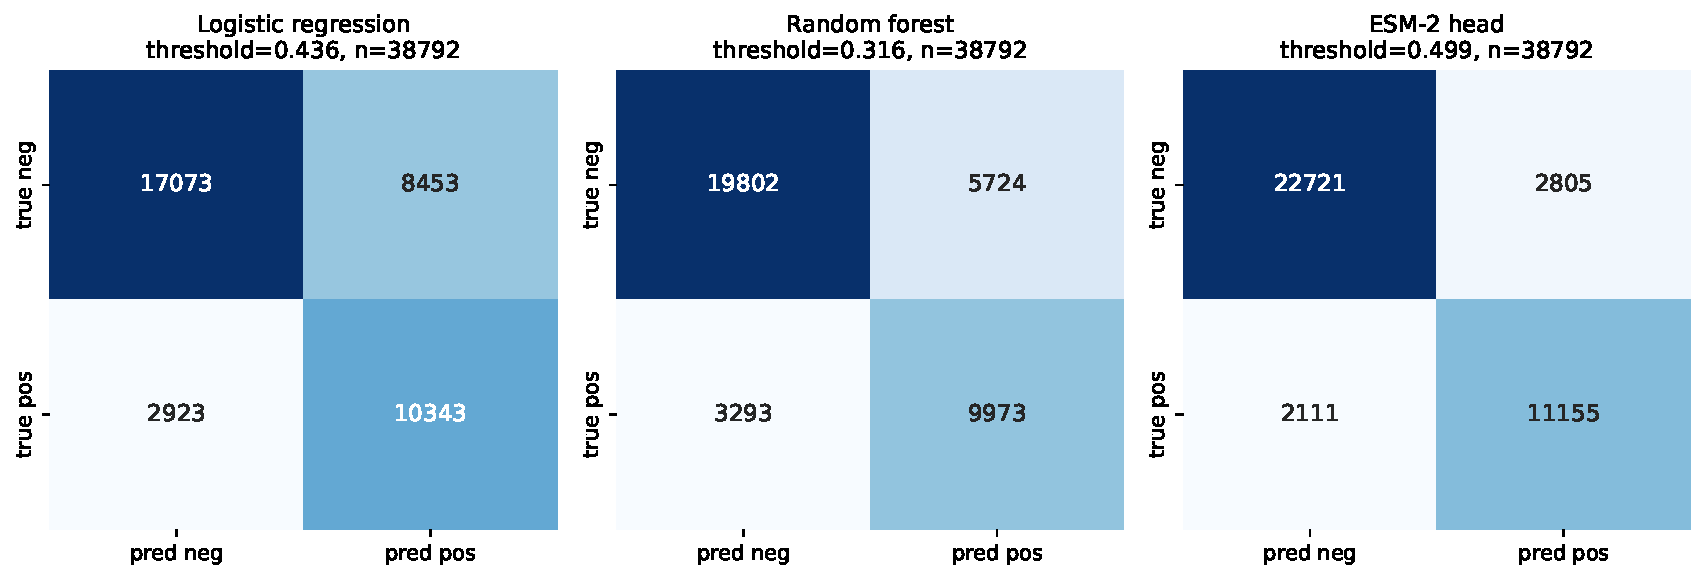
\includegraphics[width=\linewidth]{../figures/fig3_confusion.pdf}
\caption{\textbf{Confusion matrices on the test set (Figure 3).} Each panel uses its model's val-tuned operating threshold. The ESM-2 head reduces both false negatives and false positives compared with the handcrafted baselines.}
\label{fig:confusion}
\end{figure}

\begin{figure}[t]
\centering
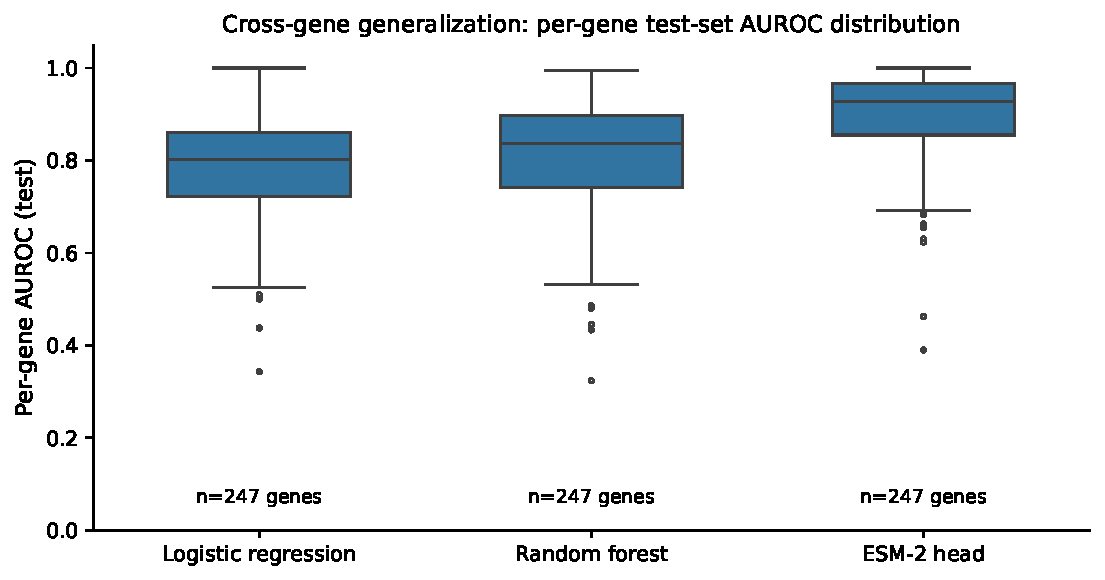
\includegraphics[width=0.95\linewidth]{../figures/fig6_per_gene_auroc.pdf}
\caption{\textbf{Per-gene test AUROC distribution (Figure 6).} Each box summarizes per-gene AUROCs across the 247 test genes that have $\geq 5$ pathogenic and $\geq 5$ benign variants. Higher is better. The ESM-2 head's median and lower whisker are both above those of the handcrafted baselines, indicating the improvement is broad-based across genes rather than concentrated in a few.}
\label{fig:pergene}
\end{figure}

\section*{Discussion}

\textbf{Direct numerical answers to the two questions the proposal poses.}
(i) \emph{How much pathogenicity signal do simple interpretable features capture on cross-gene tests?} The L2 logistic regression already reaches AUROC $0.80$, and a random forest on the same five feature families reaches AUROC $0.85$ / AUPRC $0.76$. Roughly \textbf{nine-tenths of ESM-2's AUROC and 85\% of its AUPRC} is recovered by hand-engineered features that fit in 62 dimensions, train in under two seconds, and can be interpreted variable by variable (Appendix Figure~\ref{fig:featimp}). (ii) \emph{Does ESM-2 improve cross-gene generalization beyond handcrafted features?} Yes: $+0.089$ AUROC and $+0.137$ AUPRC over the random forest, with bootstrap CIs that do not overlap, on genes that were entirely absent from training. The Appendix studiedness analysis (Figure~\ref{fig:studiedness}) shows the ESM-2 advantage is roughly stable across well- and poorly-studied genes -- the gain is unlikely to be entirely an artifact of pretraining contamination, though we cannot rule out a small contribution.

\textbf{The four-dimensional tradeoff.} Logistic regression is the simplest and most interpretable (62 coefficients, 1\,KB on disk, 0.04\,ms per variant) but the weakest. Random forest is interpretable through feature importances, lands midway in performance, but its 500-tree ensemble bloats to 2.4\,GB on disk and 46\,ms per variant. The ESM-2 head trains in 16\,s on top of 4\,minutes of one-time embedding extraction, occupies 4\,MB on disk, and runs at 0.2\,ms per variant -- but its inputs are opaque 1280-d vectors. Interpretability and predictive performance pull in opposite directions even before the AlphaMissense reference is reached.

\textbf{Limitations.} (1) We use only the canonical UniProt isoform per gene; 13{,}364 variants whose ClinVar transcript referenced a non-canonical isoform were dropped at the ref-AA verification step. (2) ESM-2 was pretrained on UR50 which contains human proteins, so some metric inflation is plausible; our studiedness analysis is a proxy and not a true ablation. (3) AlphaMissense and CADD likely share training data with ClinVar; their test scores should be read as upper-bound references, not as a fair head-to-head. (4) F1 thresholds were tuned on val; reporting AUPRC and AUROC keeps the headline conclusion threshold-free.

\textbf{Future directions.} A natural next step is to combine handcrafted features with ESM-2 embeddings in a single linear probe, which would isolate how much extra signal each side contributes; another is to fine-tune ESM-2 on ClinVar end-to-end and quantify how much performance comes from the embeddings versus the small head.

\section*{Supplementary materials}
The supplementary archive \texttt{supplementary\_team19\_gi2100\_vsj7589.zip} contains the full source tree (\texttt{src/imc/}, \texttt{scripts/}, \texttt{configs/}), pinned dependencies (\texttt{requirements.txt}), the reproduction guide (\texttt{REPRODUCE.md}), data download instructions (\texttt{data/README.md}), and the generated figures and tables (\texttt{reports/figures/}, \texttt{reports/tables/}). The full pipeline can be reproduced end-to-end with \texttt{make reproduce}; resumable checkpoints make every long-running step (ESM-2 embedding extraction, MLP head training) safe to interrupt and restart. The repository is at \url{https://github.com/GeorgiosIoannouCoder/interpretable-missense-classification}.

\bibliographystyle{plainnat}
\bibliography{references}

\appendix
\section*{Appendix}

\begin{table}[h]
\centering
\small
\caption{\textbf{Table 1 / Filtering funnel.} Each row reports retained ClinVar variants after applying the labelled stage. The proposal's cited 2026-03-30 baseline (4.24\,M variation records) is reproduced approximately at the GRCh38 stage with our 2026-05-04 snapshot.}
\label{tab:funnel}
\begin{tabular}{lr}
\toprule
\textbf{Stage} & \textbf{Variants retained} \\
\midrule
Raw \texttt{variant\_summary.txt} rows                      & 8{,}978{,}110 \\
After Assembly = GRCh38                                     & 4{,}455{,}427 \\
After germline only                                         & 4{,}142{,}993 \\
After single-nucleotide variant type                        & 3{,}859{,}832 \\
After missense parse                                        & 2{,}415{,}038 \\
After P/LP or B/LB label only                               &   210{,}038 \\
After dedup by (transcript, AA pos, ref AA, alt AA)         &   208{,}490 \\
After UniProt Swiss-Prot mapping with ref-AA verification   &   193{,}483 \\
\bottomrule
\end{tabular}
\end{table}

\begin{table}[h]
\centering
\small
\caption{\textbf{Table A1 / Computational-simplicity (efficiency) per model.} Inference latency measured per variant on the GH200 (CPU for sklearn models, GPU for the ESM-2 head -- excluding the one-time 4\,minutes of embedding extraction).}
\label{tab:efficiency}
\begin{tabular}{lrrrr}
\toprule
\textbf{Model} & \textbf{Params} & \textbf{Disk size (MB)} & \textbf{Train time (s)} & \textbf{Inference (ms / variant)} \\
\midrule
Logistic regression & 63       & 0.001          & 0.4          & 0.04 \\
Random forest       & 500 trees & 2{,}412.7      & 1.8          & 45.7 \\
ESM-2 head          & 331{,}265 & 3.8            & 16.5         & 0.2  \\
\bottomrule
\end{tabular}
\end{table}

\begin{figure}[h]
\centering
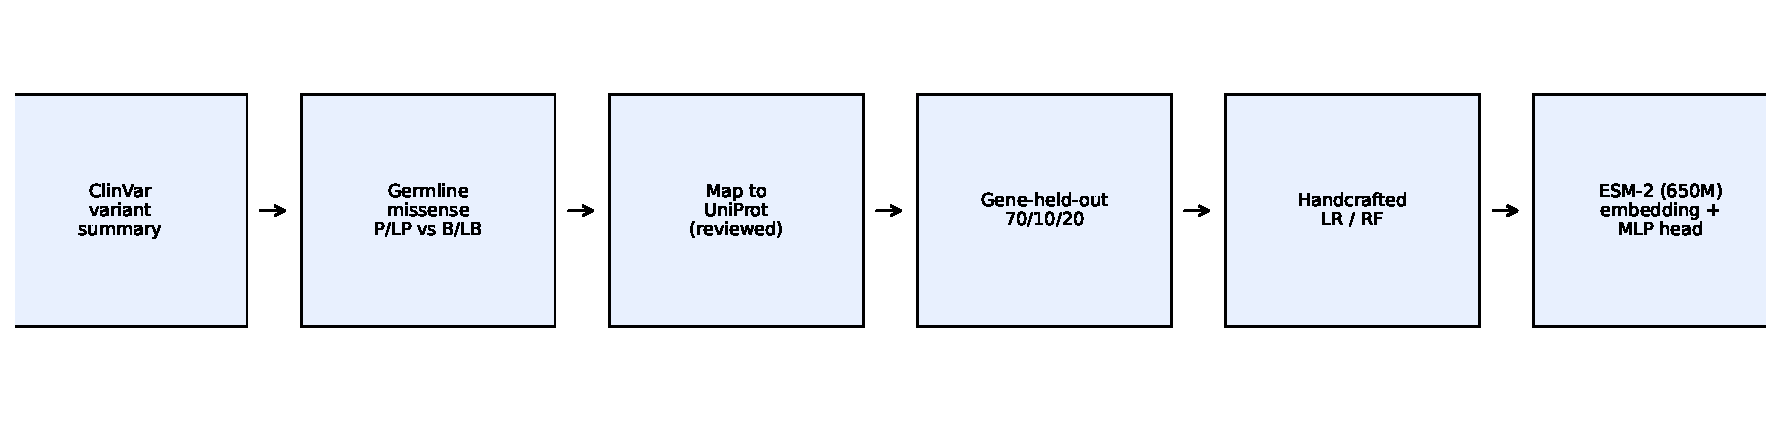
\includegraphics[width=\linewidth]{../figures/fig1_pipeline.pdf}
\caption{\textbf{Figure 1 / Pipeline schematic.} Data flow from raw ClinVar to the gene-held-out evaluation.}
\label{fig:pipeline}
\end{figure}

\begin{figure}[h]
\centering
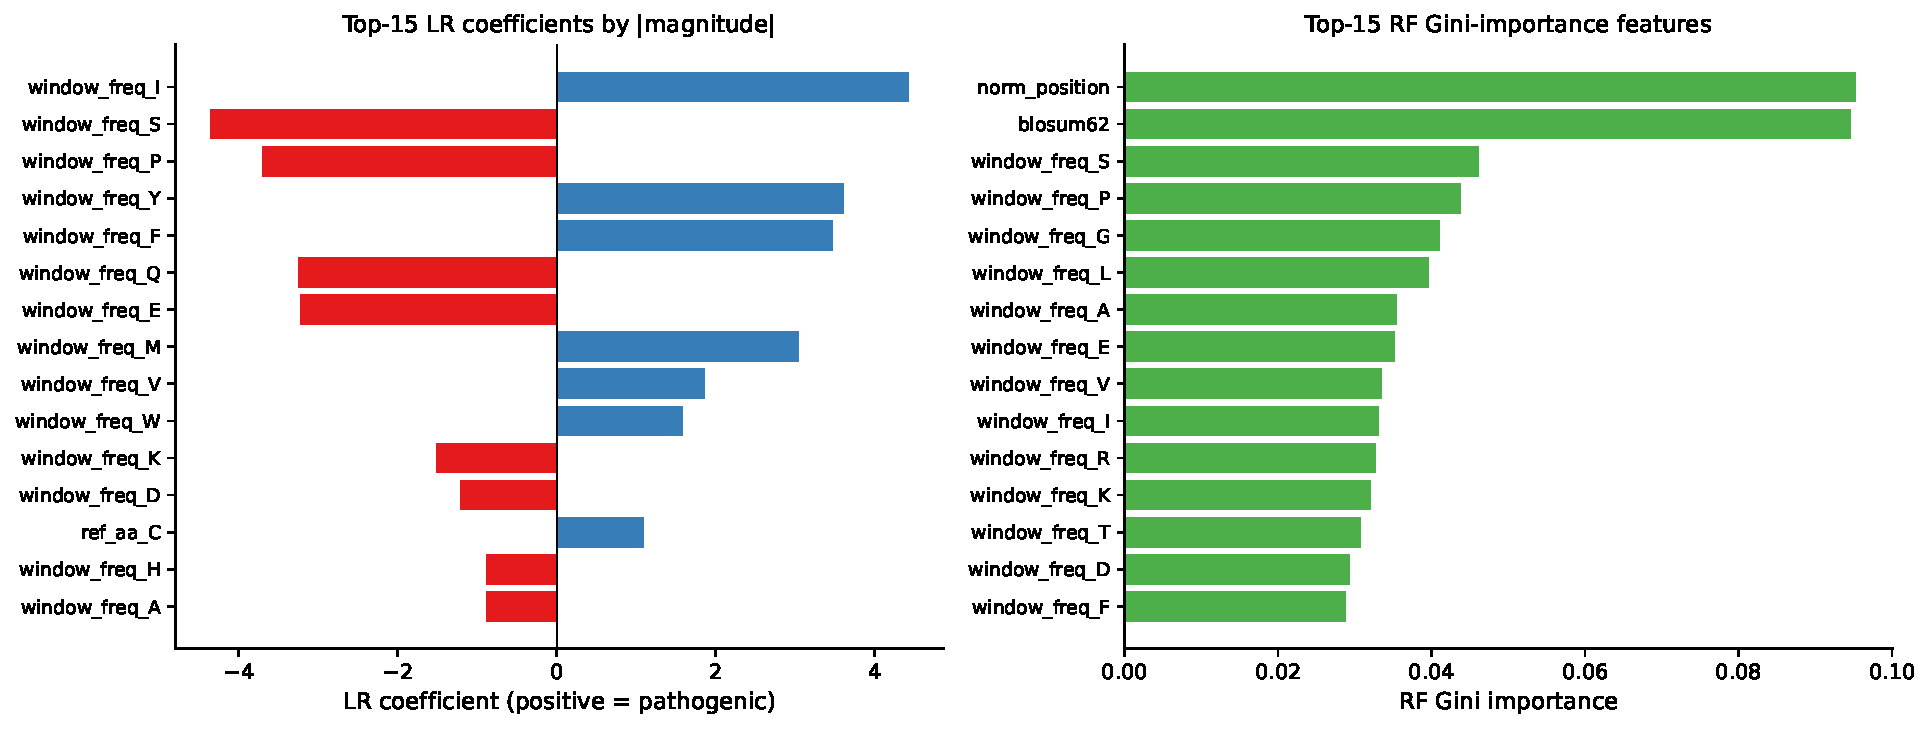
\includegraphics[width=\linewidth]{../figures/fig4_feature_importance.pdf}
\caption{\textbf{Figure 4 / Handcrafted-feature interpretability.} Top-15 LR coefficients (left) and top-15 RF Gini importances (right). The most influential features are alternate amino acids (Cys, Gly, Pro, Trp), the BLOSUM62 score, and one-hot reference amino acids -- all biologically expected.}
\label{fig:featimp}
\end{figure}

\begin{figure}[h]
\centering
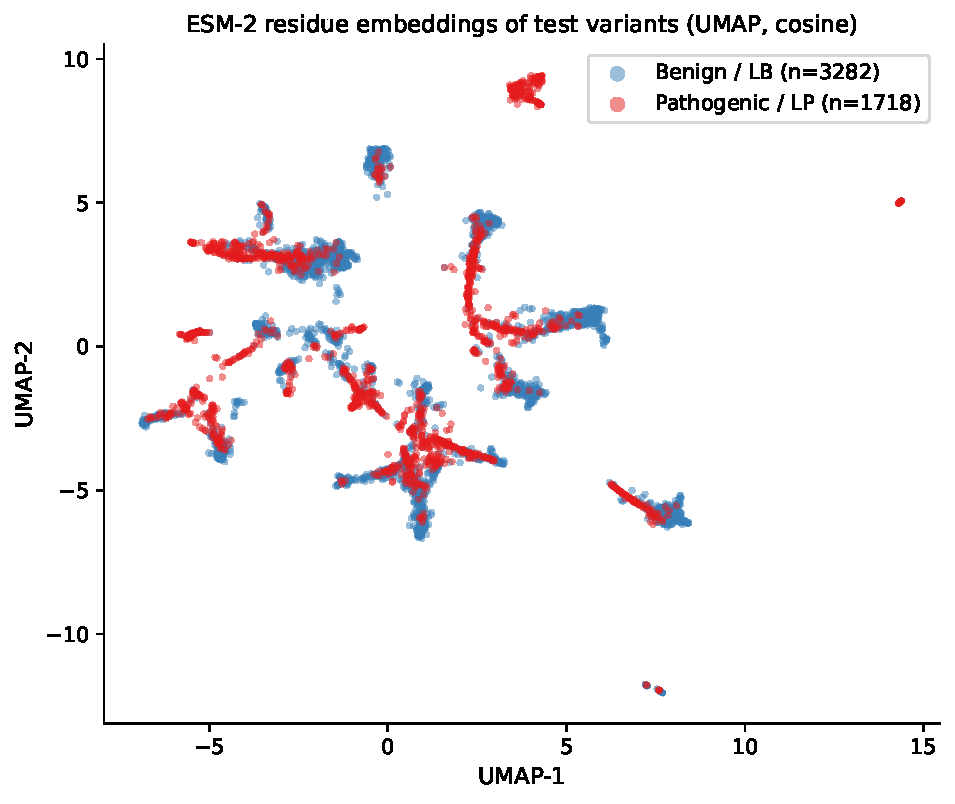
\includegraphics[width=0.85\linewidth]{../figures/fig5_umap.pdf}
\caption{\textbf{Figure 5 / UMAP of ESM-2 test embeddings.} A 5{,}000-variant random subsample of the test set, colored by ClinVar label. Pathogenic and benign clouds are partly separable in the embedding space even before any classifier is trained -- the head's job is largely a linear cleanup.}
\label{fig:umap}
\end{figure}

\begin{figure}[h]
\centering
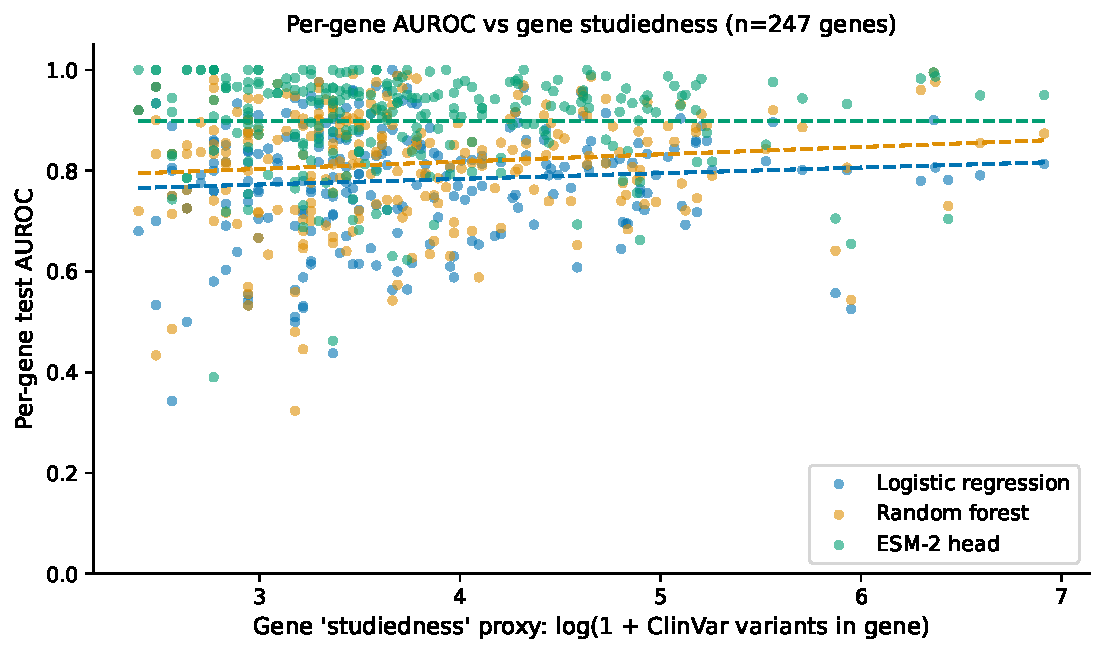
\includegraphics[width=0.85\linewidth]{../figures/fig7_studiedness.pdf}
\caption{\textbf{Figure 7 / Per-gene AUROC vs gene studiedness.} A linear fit of per-gene AUROC versus $\log(1 + \text{ClinVar variants per gene})$ (a proxy for how heavily a gene is studied). The ESM-2 head's slope is not noticeably steeper than the baselines', suggesting its advantage is broadly distributed rather than concentrated on well-represented genes.}
\label{fig:studiedness}
\end{figure}

\begin{figure}[h]
\centering
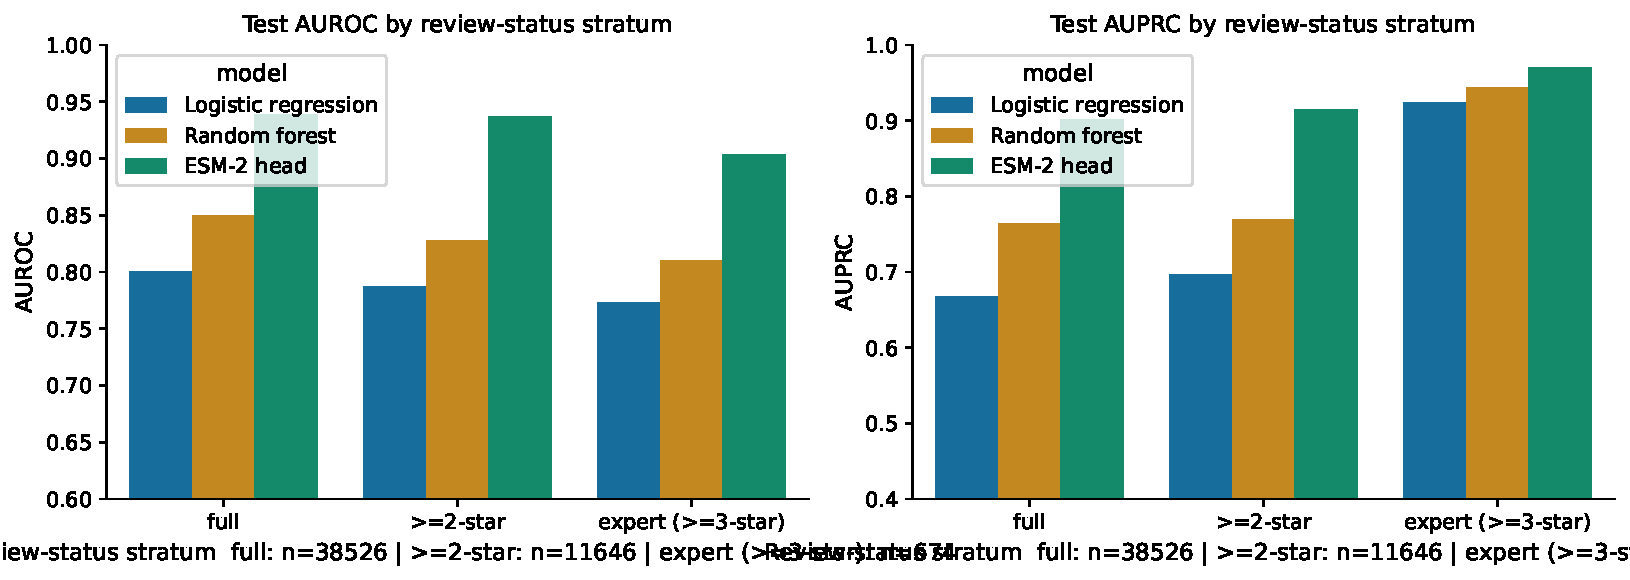
\includegraphics[width=\linewidth]{../figures/fig8_review_status.pdf}
\caption{\textbf{Figure 8 / Review-status sensitivity.} Test AUROC and AUPRC stratified by ClinVar review-status confidence: full retained set, $\geq$2-star (criteria, multiple submitters, no conflicts), and expert ($\geq$3-star: reviewed by expert panel or practice guideline). Conclusions hold across strata; the small expert-only stratum is more variable.}
\label{fig:reviewstatus}
\end{figure}

\end{document}
